\section{Grammatical approach}
\label{gramap}

A natural way to map questions into normal forms is to analyse the grammatical structure of the sentence. Some algorithms use the concrete syntax tree (or parse tree) representation to perform this task (\cite{parsetree} or \cite{parsetree2}). Another popular representation is the dependency tree. This structure describes grammatical relationships between the words of the sentence. Although the dependency tree is often used in Question Answering (\cite{Zouaq1} and \cite{Zouaq2}), algorithms for producing triples from it are pretty rare and poorly described.

The aim of this module is to provide a full algorithm that maps questions into normal forms, mainly using the dependency tree representation output by the Stanford Parser (see \cite{stanfordmanual}). We will focus on factoid \textit{wh-}questions.

%########################################################################################%

\subsection{Methods}
\label{met}

The normal form is obtained by applying some operations on the dependency tree output by the Stanford Parser. We detail throughout this section the different steps of our algorithm and we apply them on the example:
\begin{center}
 \textit{Where was the president of the United States born?}
\end{center}

%#############################################################################################################%

\subsubsection{Stanford dependency tree}
\label{sdt}

The Stanford Parser\footnote{\url{http://nlp.stanford.edu/software/corenlp.shtml}} is a natural language parser developed by the \emph{Stanford Natural Language Processing Group}. It is well-documented and considered as a ``state of the art'' program. The Stanford Parser provides classical tools of NLP theory (part-of-speech  tagger, named-entity recognizer, constituency parser, etc.) but also a very powerful dependency parser.

A dependency tree reflects the grammatical relationships between words in a sentence. Figure \ref{tree_one} provides an overview of such a tree in our example. For instance, the edge:
  \[\texttt{president}\xrightarrow{\texttt{det}}\texttt{the}\]
means that \emph{the} is a determiner for \emph{president}.

\begin{figure}
  \centering
    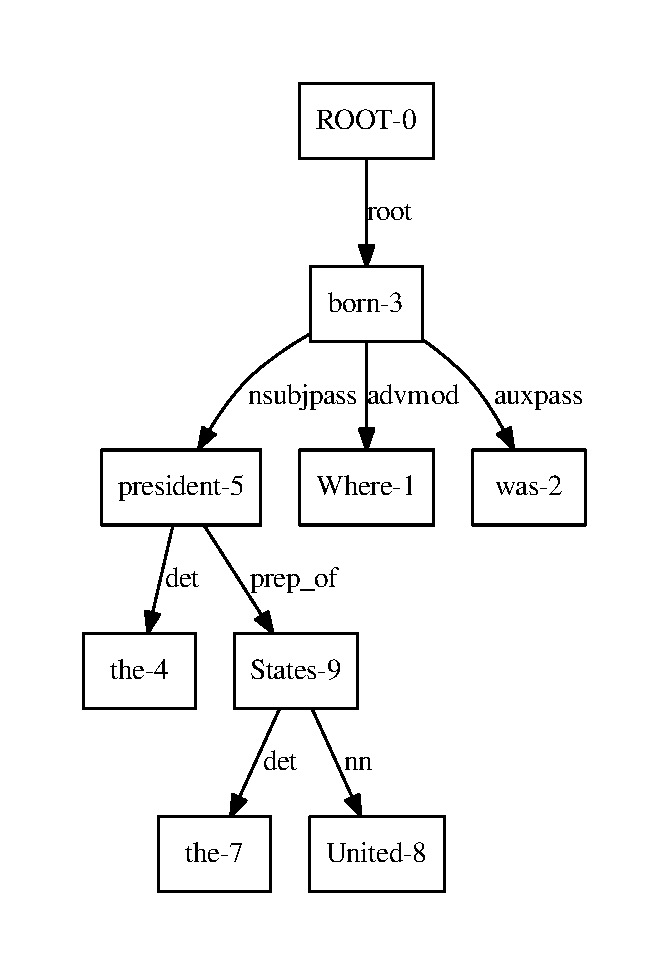
\includegraphics[scale=0.6]{../examples_NLP_grammatical/tree1bis.pdf}
  \caption{Dependency tree of \emph{Where was the president of the United States born?}}
  \label{tree_one}
\end{figure}

The Stanford typed dependencies manual (\cite{stanfordmanual}) details the full list and description of possible grammatical dependencies.

%#############################################################################################################%

\subsubsection{Dependency tree simplification}
\label{dts}

The simplification of the dependency tree consists of several operations applied on the tree to change its shape and prepare the production of the normal form. At the end of the simplification, all the dependency tags (the Stanford Parser uses more than 50 grammatical dependency tags) have been replaced by a small subset of eight (new) tags.

%-------------------------------------------------------------------------------------------------------------%

\paragraph{Preprocessing}
\label{pre}

First of all, we perform multiword expressions recognition in order to merge all the nodes of the tree that belong to a same expression. We merge especially neighbour nodes with a same named-entity tag (for instance, \textit{United} and \textit{States} are tagged \texttt{LOCATION} and therefore merged into \textit{United States}). Other kinds of merging are performed in section \ref{lot}, using the grammatical dependencies.

Then, the question word (Who, Where, How tall, etc.) is identified and removed from the dependency tree (it will be used later to build and improve the normal form). This operation is performed using a list of about 30 question words and looking at the two first words of the sentence (they are supposed to contain the question word).

Finally, lemmatization is applied on nouns (e.g. \textit{presidents} is mapped to \textit{president}) and nounification on verbs (e.g. \textit{born} is mapped to \textit{birth}).

Preprocessing is illustrated in figure \ref{tree_two}.

\begin{figure}
  \centering
    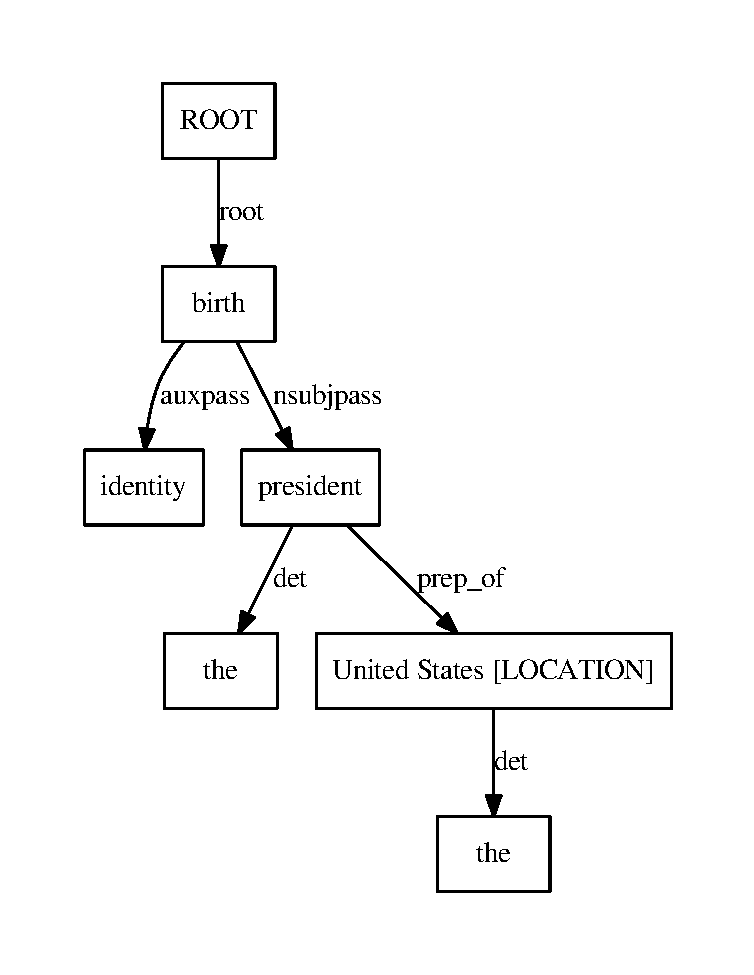
\includegraphics[scale=0.6]{../examples_NLP_grammatical/tree2bis.pdf}
  \caption{Preprocessed dependency tree of \emph{Where was the president of the United States born?}}
  \label{tree_two}
\end{figure}

%-------------------------------------------------------------------------------------------------------------%

\paragraph{Global transformations}
\label{glt}

Two kinds of transformations modify the global shape of the tree. These operations are applied for \texttt{amod} dependencies if the output node of the dependency edge is a leaf and has a JJS (superlative) or ORDINAL part-of-speech (POS) tag. They are also applied for \texttt{conj} dependencies. 

Global transformations add a new node and re-balance the tree. Figure \ref{ands} illustrates the transformation applied for conjunction dependencies (\texttt{conj\_or}, \texttt{conj\_and}, etc.). Figure \ref{amods} gives the transformation for an \texttt{amod} dependency (the POS tag of \textit{highest} is JJS).

\begin{figure}
\[ \begin{matrix} 
      \begin{tikzpicture}
        \node (1) at (10,10) {$N_1$};
        \node (2) at (8,8.5) {$N_2$};
        \node (3) at (8,7.5) {$T_2$};
        \node (4) at (12,8.5) {$T_3$};

        \draw[->, >=latex] (1) edge node[sloped, anchor=center, above] {} (4);
        \draw[->, >=latex] (2) edge node[sloped, anchor=center, above] {} (3);
        \draw[->, >=latex] (1) edge node[sloped, anchor=center, above] {conj\_or} (2);
      \end{tikzpicture}
     \end{matrix} \quad \rightsquigarrow \quad 
  \begin{matrix} 
      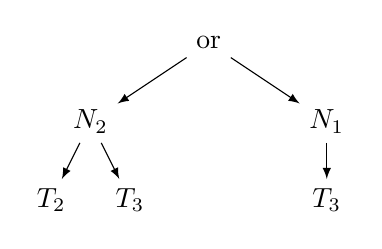
\begin{tikzpicture}
        \node (0) at (10,10) {or};
        \node (1) at (11.5,9) {$N_1$};
        \node (2) at (8.5,9) {$N_2$};
        \node (3) at (8,8) {$T_2$};
        \node (4) at (11.5,8) {$T_3$};
        \node (5) at (9,8) {$T_3$};

        \draw[->, >=latex] (0) edge node[sloped, anchor=center, above] {} (1);
        \draw[->, >=latex] (0) edge node[sloped, anchor=center, above] {} (2);
        \draw[->, >=latex] (1) edge node[sloped, anchor=center, above] {} (4);
        \draw[->, >=latex] (2) edge node[sloped, anchor=center, above] {} (5);
        \draw[->, >=latex]  (2) edge node[sloped, anchor=center, above] {} (3);
      \end{tikzpicture}
     \end{matrix} \]
  \caption{Remove \texttt{conj\_or} dependencies}
  \label{ands}
\end{figure}

%-------------------------------------------------------------------------------------------------------------%

\paragraph{Local transformations}
\label{lot}

\begin{figure}
\[ \begin{matrix} 
      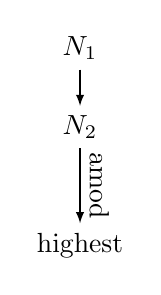
\begin{tikzpicture}
        \node (1) at (10,10) {$N_1$};
        \node (2) at (10,9) {$N_2$};
        \node (3) at (10,7.5) {highest};
        
        \draw[->, >=latex] (1) edge node[sloped, anchor=center, above] {} (2);
        \draw[->, >=latex] (2) edge node[sloped, anchor=center, above] {amod} (3);
      \end{tikzpicture}
     \end{matrix} \quad \rightsquigarrow \quad 
  \begin{matrix} 
      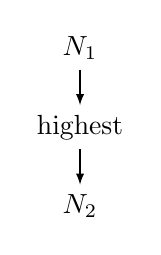
\begin{tikzpicture}
        \node (1) at (10,10) {$N_1$};
        \node (2) at (10,8) {$N_2$};
        \node (3) at (10,9) {highest};
        
        \draw[->, >=latex] (1) edge node[sloped, anchor=center, above] {} (3);
        \draw[->, >=latex] (3) edge node[sloped, anchor=center, above] {} (2);
      \end{tikzpicture}
     \end{matrix} \]
  \caption{Remove \texttt{amod} dependencies}
  \label{amods}
\end{figure}

Finally, all remaining edges are analysed locally. We apply one of the following rule to each of them, depending on their dependency tags:
\begin{itemize}
 \item \textbf{Merge} the two endpoints of the edge. It is a new step of multiword expressions merging. This rule is applied for \texttt{nn} dependencies for example:
 \[ \texttt{birth}\xrightarrow{\texttt{nn}}\texttt{date} \qquad \text{becomes:} \qquad \texttt{birth date}\]
 
 \item \textbf{Remove} the sub tree pointed out by the edge. This rule is applied for \texttt{det} dependencies for example:
 \[ \texttt{president}\xrightarrow{\texttt{det}}\texttt{the} \qquad \text{becomes:} \qquad \texttt{president}\]
 
 \item \textbf{Replace} the dependency tag by a \textit{triple production tag}. We have currently defined eight different types of \textit{triple production tags}: $R_0, \cdots, R_5, R_{spl}, R_{conj}$. These tags are used to produce the final result. We attribute the same tag to dependency relationships that must produce the same type of nodes or connectors in the normal form. For instance, we replace \texttt{prep} and \texttt{poss} dependencies by the tag $R_5$:
 \[ \texttt{president} \xrightarrow{\texttt{prep\_of}} \texttt{France} \qquad \text{becomes:} \qquad \texttt{president} \xrightarrow{R_5} \texttt{France}\] 
\end{itemize}

Finally, depending on the question word we add some information in certain nodes (for instance, if the question word is \textit{where} we try to add the word \textit{place} into the child of the root of the tree). This extra transformation is supported actually for about 30 question words.

Figure \ref{tree_three} illustrates the dependency tree simplification applied on our example.

\begin{figure}
  \centering
    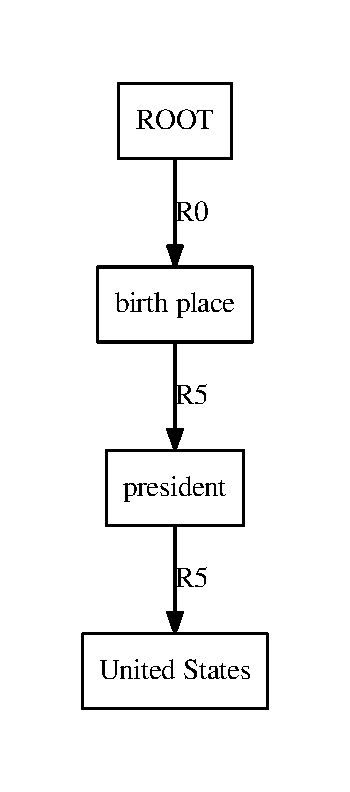
\includegraphics[scale=0.6]{../examples_NLP_grammatical/tree3bis.pdf}
  \caption{Simplified dependency tree of \emph{Where was the president of the United States born?}}
  \label{tree_three}
\end{figure}

%#############################################################################################################%

\paragraph{Construction of the normal form}
\label{cot}

The final step of the algorithm maps the tree obtained at the end of section \ref{dts} to a normal form that follows the data model presented in part \ref{rdf}. The transformation is a recursive function $\produ$ that takes a tree $T$ as input and outputs the normal form. We give the main rules applied to obtain $\produ(T)$. Trees are denoted by $T_{...}$ and nodes by $N_{...}$. For a tree $T$ (resp. a node $N$), $\underline{T}$ (resp. $\underline{N}$) represents the words contained in the root of $T$ (resp. in $N$).

First of all, if $N$ is a leaf then $\produ(N) = \underline{N}$ (\textit{value} node).

Then, rules $R_0$ to $R_5$ are used to produce the different types of possible triples. Table \ref{normtab} gives $\produ(N \xrightarrow{R_i} T)$ when $T$ is the only child of $N$ and $R_i \in \{R_0, \cdots, R_5\}$. For instance, $\produ(N \xrightarrow{R_3} T)$ is $\triple(?,\underline{N},\produ(T))$.

\begin{table}
  \begin{center}
    \begin{tabular}{c c}
      \hline \hline
      Rule $R$ & $\produ(N \xrightarrow{R} T)$ \\ \hline
      $R_0$    & $\produ(T)$ \rule[-7pt]{0pt}{20pt} \\
      $R_1$    & $\underline{T}$ \rule[-7pt]{0pt}{20pt} \\
      $R_2$    & $\triple(\underline{T},\underline{N},?)$ if $T$ is a leaf \rule[-7pt]{0pt}{20pt} \\
               & $\produ(T)$ otherwise \rule[-7pt]{0pt}{20pt} \\
      $R_3$    & $\triple(?,\underline{N},\produ(T))$  \rule[-7pt]{0pt}{20pt}\\
      $R_4$    & $\triple(?,\produ(T),\underline{N})$ \rule[-7pt]{0pt}{20pt}\\
      $R_5$    & $\triple(\produ(T),\underline{N},?)$ \rule[-7pt]{0pt}{20pt}\\ \hline
    \end{tabular}
  \end{center}
\caption{Normalization rules for $R0, \cdots, R_5$}
\label{normtab}
\end{table}

When the root $N$ has more than one child, all linked by a rule in $\{R_0, \cdots, R_5\}$, we apply the rule of figure \ref{normsingle}.

\begin{figure}
\[ \produ
     \begin{pmatrix} 
      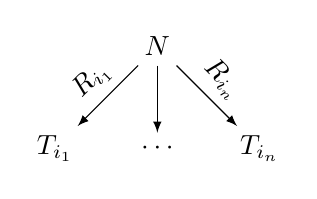
\begin{tikzpicture}
        \node (1) at (10,10.3) {$N$};
        \node (2) at (8.7,9) {$T_{i_1}$};
        \node (3) at (10,9) {$\cdots$};
        \node (4) at (11.3,9) {$T_{i_n}$};

        \draw[->, >=latex] (1) edge node[sloped, anchor=center, above] {$R_{i_1}$} (2);
        \draw[->, >=latex] (1) edge node[sloped, anchor=center, above] {} (3);
        \draw[->, >=latex] (1) edge node[sloped, anchor=center, above] {$R_{i_n}$} (4);
      \end{tikzpicture}
     \end{pmatrix} = 
     \begin{matrix}
       \bigcap\left(\produ(N \xrightarrow{R_{i_1}} T_{i_1}), \cdots, \produ(N \xrightarrow{R_{i_n}} T_{i_n}) \right)   
     \end{matrix} \]
\caption{Normalization rule for $R0, \cdots, R_5$ ($(R_{i_1}, \cdots, R_{i_n} \in \{R_0, \cdots, R_5\})$)}
\label{normsingle}
\end{figure}

Rules $R_{spl}$ and $R_{conj}$ are produced by the global transformations performed in part \ref{glt}. When rule $R_{spl}$ occurs, the root node contains a superlative or an ordinal and it has only one child. Depending on the superlative/ordinal (we have listed the most common ones), $\produ$ outputs the relevant connector nodes. A general example is presented in figure \ref{normspl}. Rule $R_{conj}$ is used for conjunction. A general example is presented in figure \ref{normconj}.

\begin{figure}
\[ \produ
     \begin{pmatrix} 
       \text{biggest} \xrightarrow{R_{spl}} T
     \end{pmatrix} =
     \begin{matrix}
      \begin{tikzpicture}
        \node (1) at (10,9.5) {$\last$};
        \node (2) at (10,8.5) {$\sort$};
        \node (8) at (11.5,7) {size};
        \node (9) at (8.5,7) {$\produ(T)$};

        \draw[->, >=latex] (1) edge node[sloped, anchor=center, above] {} (2);
        \draw[->, >=latex] (2) edge node[sloped, anchor=center, above] {\scriptsize{resource}} (8);
        \draw[->, >=latex] (2) edge node[sloped, anchor=center, above] {\scriptsize{list}} (9);
      \end{tikzpicture}
     \end{matrix} \]
\caption{Normalization rule for $R_{spl}$}
\label{normspl}
\end{figure}

\begin{figure}
\[\produ
    \begin{pmatrix} 
      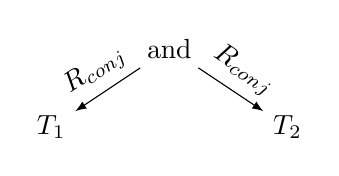
\begin{tikzpicture}
        \node (1) at (10,10) {and};
        \node (2) at (8.5,9) {$T_1$};
        \node (3) at (11.5,9) {$T_2$};

        \draw[->, >=latex] (1) edge node[sloped, anchor=center, above] {$R_{conj}$} (2);
        \draw[->, >=latex] (1) edge node[sloped, anchor=center, above] {$R_{conj}$} (3);
      \end{tikzpicture} 
    \end{pmatrix} =
    \begin{matrix}
      \begin{tikzpicture}
        \node (1) at (10,10) {$\cap$};
        \node (2) at (8,9) {$\produ(T_1)$};
        \node (3) at (12,9) {$\produ(T_2)$};

        \draw[->, >=latex] (1) edge node[sloped, anchor=center, above] {} (2);
        \draw[->, >=latex] (1) edge node[sloped, anchor=center, above] {} (3);
      \end{tikzpicture}
    \end{matrix} \]
\caption{Normalization rule for $R_{conj}$}
\label{normconj}
\end{figure}

All the rules we use are available in our implementation\footnote{\url{https://github.com/ProjetPP/PPP-QuestionParsing-Grammatical}\label{firstf}}. Figure \ref{normal1} gives a possible normal form obtained in our example.

\begin{figure}%[H] % <================== H
 \centering
  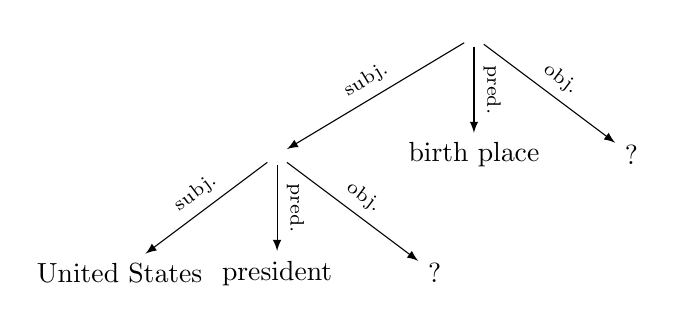
\begin{tikzpicture}
    \node (2) at (11,8.5) {$\triple$};
    \node (3) at (11,7) {birth place};
    \node (4) at (13,7) {?};
    \node (5) at (8.5,7) {$\triple$};
    \node (6) at (6.5,5.5) {United States};
    \node (7) at (8.5,5.5) {president};
    \node (8) at (10.5,5.5) {?};

    \draw[->, >=latex] (2) edge node[sloped, anchor=center, above] {\scriptsize{pred.}} (3);
    \draw[->, >=latex] (2) edge node[sloped, anchor=center, above] {\scriptsize{obj.}} (4);
    \draw[->, >=latex] (2) edge node[sloped, anchor=center, above] {\scriptsize{subj.}} (5);
    \draw[->, >=latex] (5) edge node[sloped, anchor=center, above] {\scriptsize{subj.}} (6);
    \draw[->, >=latex] (5) edge node[sloped, anchor=center, above] {\scriptsize{pred.}} (7);
    \draw[->, >=latex] (5) edge node[sloped, anchor=center, above] {\scriptsize{obj.}} (8);
  \end{tikzpicture}
 \caption{Possible normal form for \emph{Where was the president of the United States born?}}
 \label{normal1}
\end{figure}

%#############################################################################################################%
%#############################################################################################################%

\subsection{Results and discussion}

The previous algorithm has been implemented in Python 3. We use the collapsed dependency tree output by the \textit{CoreNLP} parser with the flag \texttt{-makeCopulaHead}. We access \textit{CoreNLP} using a Python wrapper\footnote{\url{https://bitbucket.org/ProgVal/corenlp-python/overview}} we have patched to support Python 3. The code is available online\textsuperscript{\ref{firstf}}. It includes a documentation and demo files that allow the user to quickly test the algorithm. Moreover, when the user enters a question in our search engine, he can get the answer and visualise the normal form by clicking on the \texttt{Show internal results} button.

We have displayed in figure \ref{exparsing} four normal forms produced by our algorithm on questions used in TREC-8 contest. These results are quite representative of what our tool can do and they are close to the expected normal forms. We have also noticed that our algorithm also supports some \textit{nominal sentences} such as \textit{``capital of England''}. 

These results prove the relevance of studying the dependency tree to extract triples. Indeed, it can be seen that the structure of the dependency tree is very close to the structure of the normal form we build. The constituency tree (as in \cite{parsetree} or \cite{parsetree2}) does not allow to handle as complex sentences as we do. Naturally, questions with complex grammatical structures are more likely to be misparsed. We also do not currently support all kinds of questions (Yes/No questions for instance).

\begin{figure}
  \begin{center}
    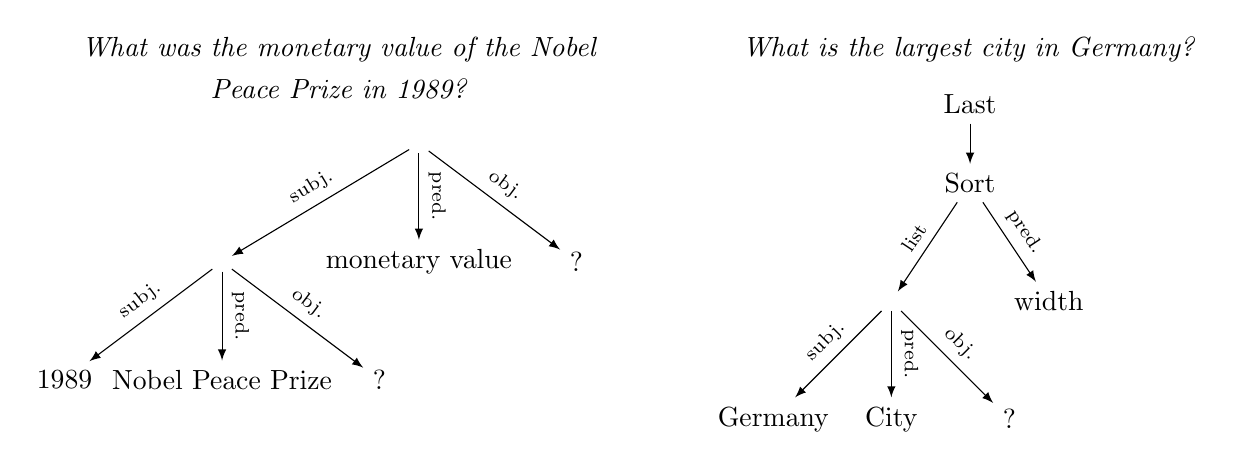
\begin{tikzpicture}
      \node (0) at (10,9.7) {\textit{What was the monetary value of the Nobel}};
      \node (1) at (10,9.2) {\textit{Peace Prize in 1989?}};
      \node (2) at (11,8.5) {$\triple$};
      \node (3) at (11,7) {monetary value};
      \node (4) at (13,7) {?};
      \node (5) at (8.5,7) {$\triple$};
      \node (6) at (6.5,5.5) {1989};
      \node (7) at (8.5,5.5) {Nobel Peace Prize};
      \node (8) at (10.5,5.5) {?};

      \draw[->, >=latex] (2) edge node[sloped, anchor=center, above] {\scriptsize{pred.}} (3);
      \draw[->, >=latex] (2) edge node[sloped, anchor=center, above] {\scriptsize{obj.}} (4);
      \draw[->, >=latex] (2) edge node[sloped, anchor=center, above] {\scriptsize{subj.}} (5);
      \draw[->, >=latex] (5) edge node[sloped, anchor=center, above] {\scriptsize{subj.}} (6);
      \draw[->, >=latex] (5) edge node[sloped, anchor=center, above] {\scriptsize{pred.}} (7);
      \draw[->, >=latex] (5) edge node[sloped, anchor=center, above] {\scriptsize{obj.}} (8);
  
      \node (9) at (18,9.7) {\textit{What is the largest city in Germany?}};
      \node (10) at (18,9) {Last};
      \node (11) at (18,8) {Sort};
      \node (12) at (19,6.5) {width};
      \node (13) at (17,6.5) {$\triple$};
      \node (14) at (15.5,5) {Germany};
      \node (15) at (17,5) {City};
      \node (16) at (18.5,5) {?};

      \draw[->, >=latex] (10) edge node[sloped, anchor=center, above] {} (11);
      \draw[->, >=latex] (11) edge node[sloped, anchor=center, above] {\scriptsize{list}} (13);
      \draw[->, >=latex] (11) edge node[sloped, anchor=center, above] {\scriptsize{pred.}} (12);
      \draw[->, >=latex] (13) edge node[sloped, anchor=center, above] {\scriptsize{subj.}} (14);
      \draw[->, >=latex] (13) edge node[sloped, anchor=center, above] {\scriptsize{pred.}} (15);
      \draw[->, >=latex] (13) edge node[sloped, anchor=center, above] {\scriptsize{obj.}} (16);
    \end{tikzpicture}
  \end{center}

  \begin{center}
    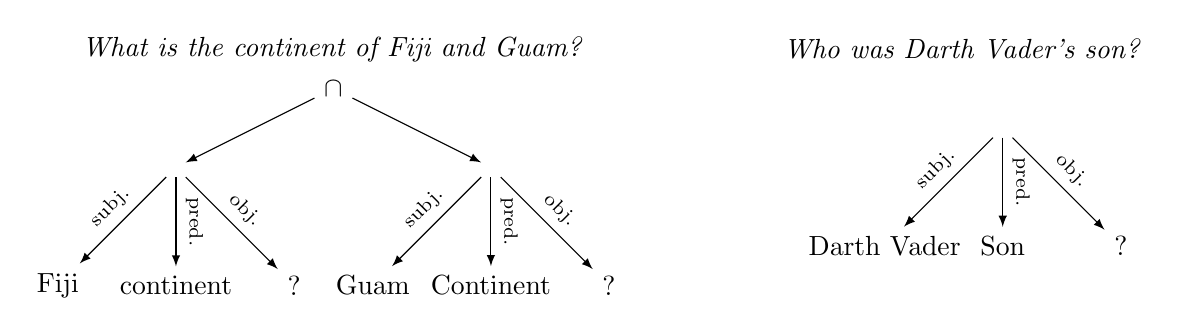
\begin{tikzpicture}
      \node (0) at (8,9.5) {\textit{What is the continent of Fiji and Guam?}};
      \node (1) at (8,9) {$\cap$};
      \node (2) at (6,8) {$\triple$};
      \node (3) at (4.5,6.5) {Fiji};
      \node (4) at (6,6.5) {continent};
      \node (5) at (7.5,6.5) {?};
      \node (6) at (10,8) {$\triple$};
      \node (7) at (8.5,6.5) {Guam};
      \node (8) at (10,6.5) {Continent};
      \node (9) at (11.5,6.5) {?};

      \draw[->, >=latex] (1) edge node[sloped, anchor=center, above] {} (2);
      \draw[->, >=latex] (1) edge node[sloped, anchor=center, above] {} (6);
      \draw[->, >=latex] (2) edge node[sloped, anchor=center, above] {\scriptsize{subj.}} (3);
      \draw[->, >=latex] (2) edge node[sloped, anchor=center, above] {\scriptsize{pred.}} (4);
      \draw[->, >=latex] (2) edge node[sloped, anchor=center, above] {\scriptsize{obj.}} (5);
      \draw[->, >=latex] (6) edge node[sloped, anchor=center, above] {\scriptsize{subj.}} (7);
      \draw[->, >=latex] (6) edge node[sloped, anchor=center, above] {\scriptsize{pred.}} (8);
      \draw[->, >=latex] (6) edge node[sloped, anchor=center, above] {\scriptsize{obj.}} (9);
  
      \node (10) at (16,9.5) {\textit{Who was Darth Vader's son?}};
      \node (11) at (16.5,8.5) {$\triple$};
      \node (12) at (15,7) {Darth Vader};
      \node (13) at (16.5,7) {Son};
      \node (14) at (18,7) {?};

      \draw[->, >=latex] (11) edge node[sloped, anchor=center, above] {\scriptsize{subj.}} (12);
      \draw[->, >=latex] (11) edge node[sloped, anchor=center, above] {\scriptsize{pred.}} (13);
      \draw[->, >=latex] (11) edge node[sloped, anchor=center, above] {\scriptsize{obj.}} (14);
    \end{tikzpicture}
  \end{center}
\caption{Example of normal forms produced by the algorithm}
\label{exparsing}
\end{figure}


%#############################################################################################################%
%#############################################################################################################%

\subsection{Future work}

Future work will consist in improving the different parts of the algorithm (multiword expressions recognition, better analysis of grammatical dependencies). We also plan to train the Stanford Parser on our own annotated data set. Moreover, our approach can be easily transposed to languages using similar grammatical dependencies than English. Finally, the extraction of triples is useful into many fields of NLP theory, other than Question Answering. For instance, our algorithm could be adapted to automatic text summarization or speech processing.
